\documentclass{article}\usepackage[]{graphicx}\usepackage[]{color}
%% maxwidth is the original width if it is less than linewidth
%% otherwise use linewidth (to make sure the graphics do not exceed the margin)
\makeatletter
\def\maxwidth{ %
  \ifdim\Gin@nat@width>\linewidth
    \linewidth
  \else
    \Gin@nat@width
  \fi
}
\makeatother

\definecolor{fgcolor}{rgb}{0.345, 0.345, 0.345}
\newcommand{\hlnum}[1]{\textcolor[rgb]{0.686,0.059,0.569}{#1}}%
\newcommand{\hlstr}[1]{\textcolor[rgb]{0.192,0.494,0.8}{#1}}%
\newcommand{\hlcom}[1]{\textcolor[rgb]{0.678,0.584,0.686}{\textit{#1}}}%
\newcommand{\hlopt}[1]{\textcolor[rgb]{0,0,0}{#1}}%
\newcommand{\hlstd}[1]{\textcolor[rgb]{0.345,0.345,0.345}{#1}}%
\newcommand{\hlkwa}[1]{\textcolor[rgb]{0.161,0.373,0.58}{\textbf{#1}}}%
\newcommand{\hlkwb}[1]{\textcolor[rgb]{0.69,0.353,0.396}{#1}}%
\newcommand{\hlkwc}[1]{\textcolor[rgb]{0.333,0.667,0.333}{#1}}%
\newcommand{\hlkwd}[1]{\textcolor[rgb]{0.737,0.353,0.396}{\textbf{#1}}}%

\usepackage{framed}
\makeatletter
\newenvironment{kframe}{%
 \def\at@end@of@kframe{}%
 \ifinner\ifhmode%
  \def\at@end@of@kframe{\end{minipage}}%
  \begin{minipage}{\columnwidth}%
 \fi\fi%
 \def\FrameCommand##1{\hskip\@totalleftmargin \hskip-\fboxsep
 \colorbox{shadecolor}{##1}\hskip-\fboxsep
     % There is no \\@totalrightmargin, so:
     \hskip-\linewidth \hskip-\@totalleftmargin \hskip\columnwidth}%
 \MakeFramed {\advance\hsize-\width
   \@totalleftmargin\z@ \linewidth\hsize
   \@setminipage}}%
 {\par\unskip\endMakeFramed%
 \at@end@of@kframe}
\makeatother

\definecolor{shadecolor}{rgb}{.97, .97, .97}
\definecolor{messagecolor}{rgb}{0, 0, 0}
\definecolor{warningcolor}{rgb}{1, 0, 1}
\definecolor{errorcolor}{rgb}{1, 0, 0}
\newenvironment{knitrout}{}{} % an empty environment to be redefined in TeX

\usepackage{alltt}
\usepackage{geometry}
\usepackage{amsmath}
\usepackage{lscape}
\geometry{verbose,tmargin=2.5cm,bmargin=2.5cm,lmargin=2.5cm,rmargin=2.5cm}
\IfFileExists{upquote.sty}{\usepackage{upquote}}{}
\begin{document}




\title{Messina E2A: Messina vs t-test}
\maketitle


%%%%%%%%%%%%%%%%%%%%%%%%%%%%%%%%%%%%%%%%%%%%%%%%%%%%%%%%%%%%%%%%%%%%%%
% LIBRARIES
%%%%%%%%%%%%%%%%%%%%%%%%%%%%%%%%%%%%%%%%%%%%%%%%%%%%%%%%%%%%%%%%%%%%%%
\section{Preparation}
\begin{knitrout}
\definecolor{shadecolor}{rgb}{0.969, 0.969, 0.969}\color{fgcolor}\begin{kframe}
\begin{alltt}
\hlkwd{library}\hlstd{(plyr)}
\hlkwd{library}\hlstd{(ggplot2)}
\end{alltt}


{\ttfamily\noindent\itshape\color{messagecolor}{\#\# Loading required package: methods}}\begin{alltt}
\hlkwd{library}\hlstd{(messina)}
\end{alltt}


{\ttfamily\noindent\itshape\color{messagecolor}{\#\# Loading required package: survival\\\#\# Loading required package: splines}}\begin{alltt}
\hlkwd{library}\hlstd{(doMC)}
\end{alltt}


{\ttfamily\noindent\itshape\color{messagecolor}{\#\# Loading required package: foreach\\\#\# Loading required package: iterators\\\#\# Loading required package: parallel}}\begin{alltt}
\hlstd{paropts} \hlkwb{=} \hlkwd{list}\hlstd{(}\hlkwc{.options.multicore} \hlstd{=} \hlkwd{list}\hlstd{(}\hlkwc{preschedule} \hlstd{=} \hlnum{FALSE}\hlstd{))}
\end{alltt}
\end{kframe}
\end{knitrout}


\begin{knitrout}
\definecolor{shadecolor}{rgb}{0.969, 0.969, 0.969}\color{fgcolor}\begin{kframe}
\begin{alltt}
\hlstd{deltaForMargin} \hlkwb{=} \hlkwa{function}\hlstd{(}\hlkwc{margin}\hlstd{,} \hlkwc{sigma_epsilon} \hlstd{=} \hlnum{1}\hlstd{,} \hlkwc{alpha} \hlstd{=} \hlnum{0.05}\hlstd{) margin} \hlopt{-} \hlnum{2}\hlopt{*}\hlstd{sigma_epsilon}\hlopt{*}\hlkwd{qnorm}\hlstd{(alpha)}
\hlstd{marginForDelta} \hlkwb{=} \hlkwa{function}\hlstd{(}\hlkwc{delta}\hlstd{,} \hlkwc{sigma_epsilon} \hlstd{=} \hlnum{1}\hlstd{,} \hlkwc{alpha} \hlstd{=} \hlnum{0.05}\hlstd{) delta} \hlopt{+} \hlnum{2}\hlopt{*}\hlstd{sigma_epsilon}\hlopt{*}\hlkwd{qnorm}\hlstd{(alpha)}

\hlstd{e2a.design} \hlkwb{=} \hlkwd{expand.grid}\hlstd{(}
        \hlkwc{Delta} \hlstd{=} \hlkwd{seq}\hlstd{(}\hlnum{0}\hlstd{,} \hlnum{5}\hlstd{,} \hlnum{0.25}\hlstd{),}
        \hlkwc{sigma_epsilon} \hlstd{=} \hlnum{1}\hlstd{,}
\hlcom{#	p1 = c(0.2, 0.5),}
\hlcom{#	pm = c(0, 0.1, 0.2),}
        \hlkwc{p1} \hlstd{=} \hlkwd{c}\hlstd{(}\hlnum{0.5}\hlstd{),}
        \hlkwc{pm} \hlstd{=} \hlkwd{c}\hlstd{(}\hlnum{0}\hlstd{),}
        \hlkwc{alpha} \hlstd{=} \hlnum{0.2}\hlstd{,}
        \hlkwc{t.alpha} \hlstd{=} \hlnum{0.05}\hlstd{,}
        \hlkwc{messina.minmarg} \hlstd{=} \hlnum{1}\hlstd{,}
        \hlkwc{messina.minsens} \hlstd{=} \hlnum{0.8}\hlstd{,}
        \hlkwc{messina.minspec} \hlstd{=} \hlnum{0.8}\hlstd{,}
        \hlkwc{n} \hlstd{=} \hlkwd{c}\hlstd{(}\hlnum{25}\hlstd{,} \hlnum{50}\hlstd{,} \hlnum{100}\hlstd{),}
        \hlkwc{reps} \hlstd{=} \hlnum{1e3}\hlstd{)}
\hlstd{e2a.design}\hlopt{$}\hlstd{margin} \hlkwb{=} \hlkwd{marginForDelta}\hlstd{(e2a.design}\hlopt{$}\hlstd{Delta, e2a.design}\hlopt{$}\hlstd{sigma_epsilon,} \hlkwc{alpha} \hlstd{= e2a.design}\hlopt{$}\hlstd{alpha)}

\hlstd{e2a.datafun} \hlkwb{=} \hlkwa{function}\hlstd{(}\hlkwc{n}\hlstd{,} \hlkwc{p1}\hlstd{,} \hlkwc{pm}\hlstd{,} \hlkwc{Delta}\hlstd{,} \hlkwc{sigma_epsilon}\hlstd{,} \hlkwc{...}\hlstd{)}
\hlstd{\{}
        \hlstd{n1} \hlkwb{=} \hlkwd{round}\hlstd{(n}\hlopt{*}\hlstd{p1)}
        \hlstd{n0} \hlkwb{=} \hlstd{n} \hlopt{-} \hlstd{n1}
        \hlstd{y} \hlkwb{=} \hlkwd{rep}\hlstd{(}\hlkwd{c}\hlstd{(}\hlnum{0}\hlstd{,} \hlnum{1}\hlstd{),} \hlkwd{c}\hlstd{(n0, n1))}
        \hlstd{y_exp} \hlkwb{=} \hlstd{y}
        \hlstd{y0x1} \hlkwb{=} \hlkwd{sample}\hlstd{((}\hlnum{1}\hlopt{:}\hlstd{n)[y} \hlopt{==} \hlnum{0}\hlstd{],} \hlkwd{floor}\hlstd{(}\hlkwd{sum}\hlstd{(y} \hlopt{==} \hlnum{0}\hlstd{)} \hlopt{*} \hlstd{pm}\hlopt{/}\hlnum{2}\hlstd{),} \hlkwc{replace} \hlstd{=} \hlnum{FALSE}\hlstd{)}
        \hlstd{y1x0} \hlkwb{=} \hlkwd{sample}\hlstd{((}\hlnum{1}\hlopt{:}\hlstd{n)[y} \hlopt{==} \hlnum{1}\hlstd{],} \hlkwd{floor}\hlstd{(}\hlkwd{sum}\hlstd{(y} \hlopt{==} \hlnum{1}\hlstd{)} \hlopt{*} \hlstd{pm}\hlopt{/}\hlnum{2}\hlstd{),} \hlkwc{replace} \hlstd{=} \hlnum{FALSE}\hlstd{)}
        \hlstd{y_exp[y0x1]} \hlkwb{=} \hlnum{1}
        \hlstd{y_exp[y1x0]} \hlkwb{=} \hlnum{0}
        \hlstd{x} \hlkwb{=} \hlstd{Delta}\hlopt{*}\hlstd{y_exp} \hlopt{+} \hlkwd{rnorm}\hlstd{(n,} \hlkwc{mean} \hlstd{=} \hlnum{0}\hlstd{,} \hlkwc{sd} \hlstd{= sigma_epsilon)}

        \hlkwd{list}\hlstd{(}\hlkwc{x} \hlstd{= x,} \hlkwc{y} \hlstd{= y,} \hlkwc{y_exp} \hlstd{= y_exp)}
\hlstd{\}}

\hlstd{e2a.detfun} \hlkwb{=} \hlkwa{function}\hlstd{(}\hlkwc{x}\hlstd{,} \hlkwc{y}\hlstd{,} \hlkwc{t.alpha}\hlstd{,} \hlkwc{messina.minsens}\hlstd{,} \hlkwc{messina.minspec}\hlstd{,} \hlkwc{messina.minmarg}\hlstd{,} \hlkwc{...}\hlstd{)}
\hlstd{\{}
        \hlstd{det.t} \hlkwb{=} \hlkwd{t.test}\hlstd{(}\hlkwc{x} \hlstd{= x[y} \hlopt{==} \hlnum{0}\hlstd{],} \hlkwc{y} \hlstd{= x[y} \hlopt{==} \hlnum{1}\hlstd{])}\hlopt{$}\hlstd{p.value} \hlopt{<} \hlstd{t.alpha}

        \hlstd{x.messina} \hlkwb{=} \hlkwd{rbind}\hlstd{(x, x)}
        \hlstd{fit.messina} \hlkwb{=} \hlkwd{messina}\hlstd{(x.messina, y} \hlopt{==} \hlnum{1}\hlstd{,} \hlkwc{min_sens} \hlstd{= messina.minsens,} \hlkwc{min_spec} \hlstd{= messina.minspec,} \hlkwc{progress} \hlstd{=} \hlnum{FALSE}\hlstd{,} \hlkwc{silent} \hlstd{=} \hlnum{TRUE}\hlstd{)}
        \hlstd{det.messina} \hlkwb{=} \hlstd{fit.messina}\hlopt{@}\hlkwc{fits}\hlopt{@}\hlkwc{summary}\hlopt{$}\hlstd{passed[}\hlnum{1}\hlstd{]} \hlopt{==} \hlnum{TRUE} \hlopt{&&} \hlstd{fit.messina}\hlopt{@}\hlkwc{fits}\hlopt{@}\hlkwc{summary}\hlopt{$}\hlstd{margin[}\hlnum{1}\hlstd{]} \hlopt{>=} \hlstd{messina.minmarg}

        \hlkwd{c}\hlstd{(}\hlkwc{t} \hlstd{= det.t,} \hlkwc{m} \hlstd{= det.messina)}
\hlstd{\}}

\hlkwd{registerDoMC}\hlstd{(}\hlnum{32}\hlstd{)}

\hlkwd{set.seed}\hlstd{(}\hlnum{20150320}\hlstd{)}
\hlstd{e2a.det} \hlkwb{=} \hlkwd{mlply}\hlstd{(e2a.design,} \hlkwa{function}\hlstd{(}\hlkwc{Delta}\hlstd{,} \hlkwc{sigma_epsilon}\hlstd{,} \hlkwc{pm}\hlstd{,} \hlkwc{p1}\hlstd{,} \hlkwc{t.alpha}\hlstd{,} \hlkwc{messina.minmarg}\hlstd{,} \hlkwc{messina.minsens}\hlstd{,} \hlkwc{messina.minspec}\hlstd{,} \hlkwc{n}\hlstd{,} \hlkwc{reps}\hlstd{,} \hlkwc{...}\hlstd{) \{}
        \hlkwd{rowMeans}\hlstd{(}\hlkwd{replicate}\hlstd{(reps, \{ data} \hlkwb{=} \hlkwd{e2a.datafun}\hlstd{(n, p1, pm, Delta, sigma_epsilon);} \hlkwd{e2a.detfun}\hlstd{(data}\hlopt{$}\hlstd{x, data}\hlopt{$}\hlstd{y, t.alpha, messina.minsens, messina.minspec, messina.minmarg) \})) \},} \hlkwc{.parallel} \hlstd{=} \hlnum{TRUE}\hlstd{,} \hlkwc{.paropts} \hlstd{= paropts)}

\hlstd{e2a.design} \hlkwb{=} \hlkwd{rbind}\hlstd{(}\hlkwd{cbind}\hlstd{(e2a.design,} \hlkwc{method} \hlstd{=} \hlstr{"t"}\hlstd{,} \hlkwc{detrate} \hlstd{=} \hlkwd{simplify2array}\hlstd{(e2a.det)[}\hlnum{1}\hlstd{,]),} \hlkwd{cbind}\hlstd{(e2a.design,} \hlkwc{method} \hlstd{=} \hlstr{"messina"}\hlstd{,} \hlkwc{detrate} \hlstd{=} \hlkwd{simplify2array}\hlstd{(e2a.det)[}\hlnum{2}\hlstd{,]))}
\end{alltt}
\end{kframe}
\end{knitrout}

\begin{knitrout}
\definecolor{shadecolor}{rgb}{0.969, 0.969, 0.969}\color{fgcolor}\begin{kframe}
\begin{alltt}
\hlcom{# ggplot(e2a.design[e2a.design$margin >= 0,], aes(x = margin, y = detrate, colour = factor(method))) + geom_line(lwd = 1) + xlab("Margin") + ylab("Detection rate") + ggtitle("Messina vs t-test") + labs(colour = "Method") + theme_bw() + facet_grid(p1 ~ pm ~ n)}
\hlcom{# ggplot(e2a.design, aes(x = margin, y = detrate, colour = factor(method))) + geom_line(lwd = 1) + xlab("Margin") + ylab("Detection rate") + ggtitle("Messina vs t-test") + labs(colour = "Method") + theme_bw() + facet_grid(p1 ~ pm ~ n)}
\hlcom{# ggplot(e2a.design, aes(x = margin, y = detrate, colour = factor(method))) + geom_line(lwd = 1) + xlab("Margin") + ylab("Detection rate") + ggtitle("Messina vs t-test") + labs(colour = "Method") + theme_bw() + facet_wrap(~ n)}
\hlstd{e2a.design}\hlopt{$}\hlstd{method} \hlkwb{=} \hlkwd{as.character}\hlstd{(e2a.design}\hlopt{$}\hlstd{method)}
\hlstd{e2a.design}\hlopt{$}\hlstd{method[e2a.design}\hlopt{$}\hlstd{method} \hlopt{==} \hlstr{"t"}\hlstd{]} \hlkwb{=} \hlstr{"t test"}
\hlstd{e2a.design}\hlopt{$}\hlstd{method[e2a.design}\hlopt{$}\hlstd{method} \hlopt{==} \hlstr{"messina"}\hlstd{]} \hlkwb{=} \hlstr{"Messina"}
\hlstd{e2a.design}\hlopt{$}\hlstd{method} \hlkwb{=} \hlkwd{as.factor}\hlstd{(e2a.design}\hlopt{$}\hlstd{method)}
\hlkwd{ggplot}\hlstd{(e2a.design[e2a.design}\hlopt{$}\hlstd{margin}\hlopt{>=}\hlnum{0}\hlstd{,],} \hlkwd{aes}\hlstd{(}\hlkwc{x} \hlstd{= margin,} \hlkwc{y} \hlstd{= detrate,} \hlkwc{colour} \hlstd{=} \hlkwd{factor}\hlstd{(method)))} \hlopt{+} \hlkwd{geom_line}\hlstd{(}\hlkwc{lwd} \hlstd{=} \hlnum{1}\hlstd{)} \hlopt{+} \hlkwd{xlab}\hlstd{(}\hlstr{"True margin"}\hlstd{)} \hlopt{+} \hlkwd{ylab}\hlstd{(}\hlstr{"Detection rate"}\hlstd{)} \hlopt{+} \hlkwd{labs}\hlstd{(}\hlkwc{colour} \hlstd{=} \hlstr{"Method"}\hlstd{)} \hlopt{+} \hlkwd{theme_bw}\hlstd{()} \hlopt{+} \hlkwd{facet_wrap}\hlstd{(}\hlopt{~} \hlstd{n)} \hlopt{+} \hlkwd{geom_vline}\hlstd{(}\hlkwc{xintercept} \hlstd{=} \hlnum{1}\hlstd{,} \hlkwc{alpha} \hlstd{=} \hlnum{0.5}\hlstd{,} \hlkwc{linetype} \hlstd{=} \hlstr{"dashed"}\hlstd{)}
\end{alltt}
\end{kframe}

{\centering 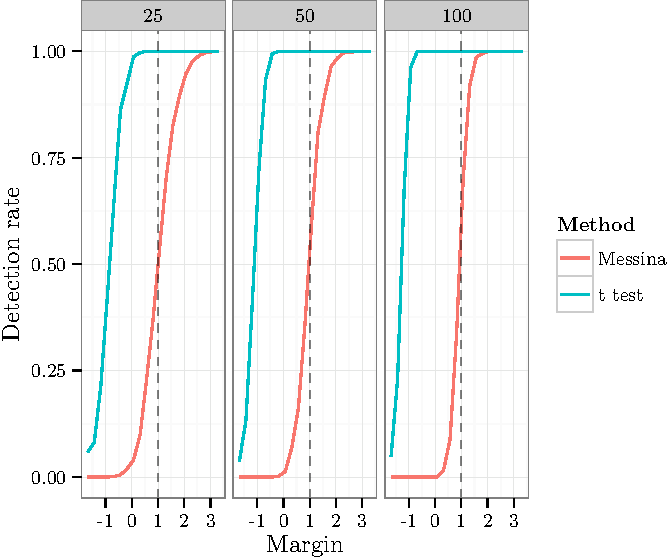
\includegraphics[width=\maxwidth]{figure/06-E2A-E2A-plots-1} 

}



\end{knitrout}

\end{document}
